\newpage
\section{Ergebnisse}
\label{sec:ergebnisse}
%Was waren die Ergebnisse der Untersuchungen?

In diesen Abschnitt werden die Ergebnisse zur Verdickungsmitteldosierung dargestellt. Nach Verifizierung des Problems und dessen Beschreibung erfolgen die Ergebnisse der Untersuchungsmethoden, sowie Entscheidungsverfahren für die Verfahrensplanung und schlussendlich die technische Umsetzung einer Dosiervariante mit einer Gefährdungsbeurteilung.

\subsection{Verifizierung und Analyse des Dosierproblems}
\label{sec:verifizierung}
Im ersten Schritt wurde der Ist-Zustand der Dosierung erfasst, sowie die Gegebenheiten im Werk analysiert. Danach erfolgte das Zusammentragen der Anforderungen an eine halbautomatisch umgesetzte Dosierung.
 
\subsubsection{Ist-Zustand: Produktionsweise und aktuelles Dosierverfahren}
Das herzustellende Produkt für das eine halbautomatische Verdickerdosierung umgesetzt werden soll nennt sich \textit{AC 548}. Es ist eine Acrylat-Copolymer Dispersion und kann als Betonschutz, Fassadenfarben, wärmeaktivierbare Klebstoffe, Putze und Buntsteinputze verwendet werden. Produziert wird \textit{AC 548} im Batch-Betrieb à \SI{14}{\tonne} und die Planung erfolgt vorzugsweise in Kampagnen. \cite{ALBO.22.02.2022} \linebreak
Derzeit wird für dieses Produkt das Verdickungsmittel Rheobyk-H 3300 VF der \textsc{Byk-Chemie GmbH} eingesetzt, welches jedoch im Laufe des Jahres 2022 durch Einstellen der Produktion mit dem Verdickungsmittel TAFIGEL PUR 85 der \textsc{Münzing Chemie GmbH} substituiert werden soll. Die aktuelle Dosierung beläuft sich dabei auf die Nutzung eines \SI{0}{\liter}-Kunststofffasses als Dosierbehälter. Hierfür werden zunächst \SI{22}{\kilo \gram} des Verdickungsmittels in einem "`Transportfass"' im Chemikalienlager abgewogen und dann am entsprechenden Einstelltank bereit gestellt. Für den Start der Dosierung wird das "`Dosierfass"', welches mit einem Dosierloch an der Fassunterseite versehen ist, in das Fallschutzgitter des Mannlochs gehängt und der Inhalt des Transportfasses in das Dosierfass gekippt. Schematisch dargestellt ist diese Dosierung in Abbildung \ref{fig:aktuelle_dosierung}.

\begin{figure}[h!]
	\centering
	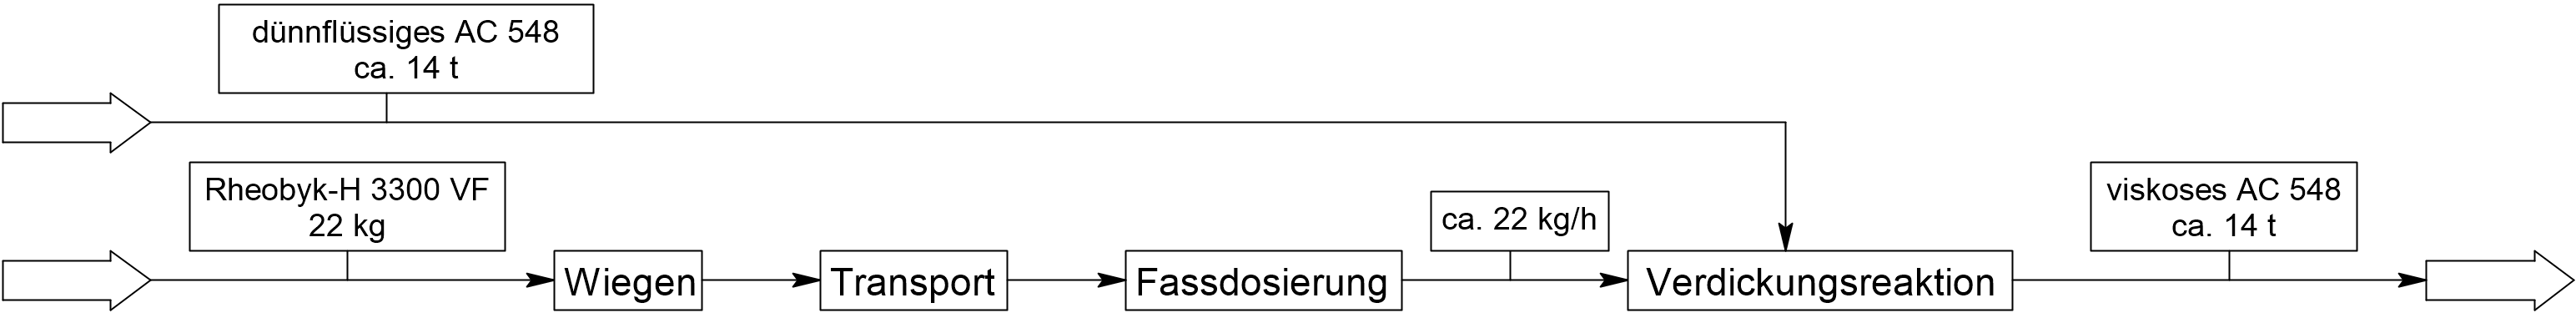
\includegraphics[width=\textwidth]{img/aktuelle_dosierung}
	\caption{Aktuelle Dosierung des Verdickungsmittels Rheobyk-H 3300 VF}
	\label{fig:aktuelle_dosierung}
\end{figure}
\FloatBarrier
%Ende

Vorteile dieses Dosierverfahrens sind die einfache und kostengünstige Umsetzung. Dem entgegen steht jedoch, dass neben dem "`Dosierloch"' und dem Fass selbst keine Einstellparameter vorhanden sind und der Dosierstrom weder messtechnisch erfasst noch im Prozessleitsystem (PLS) einsehbar ist. Zudem kann die Umsetzung für die Dosierung nur bedingt hygienisch erfolgen wie unter anderem in Abbildung \ref{fig:dosierfass} zu erkennen ist.

\begin{figure}[h!]
	\centering
	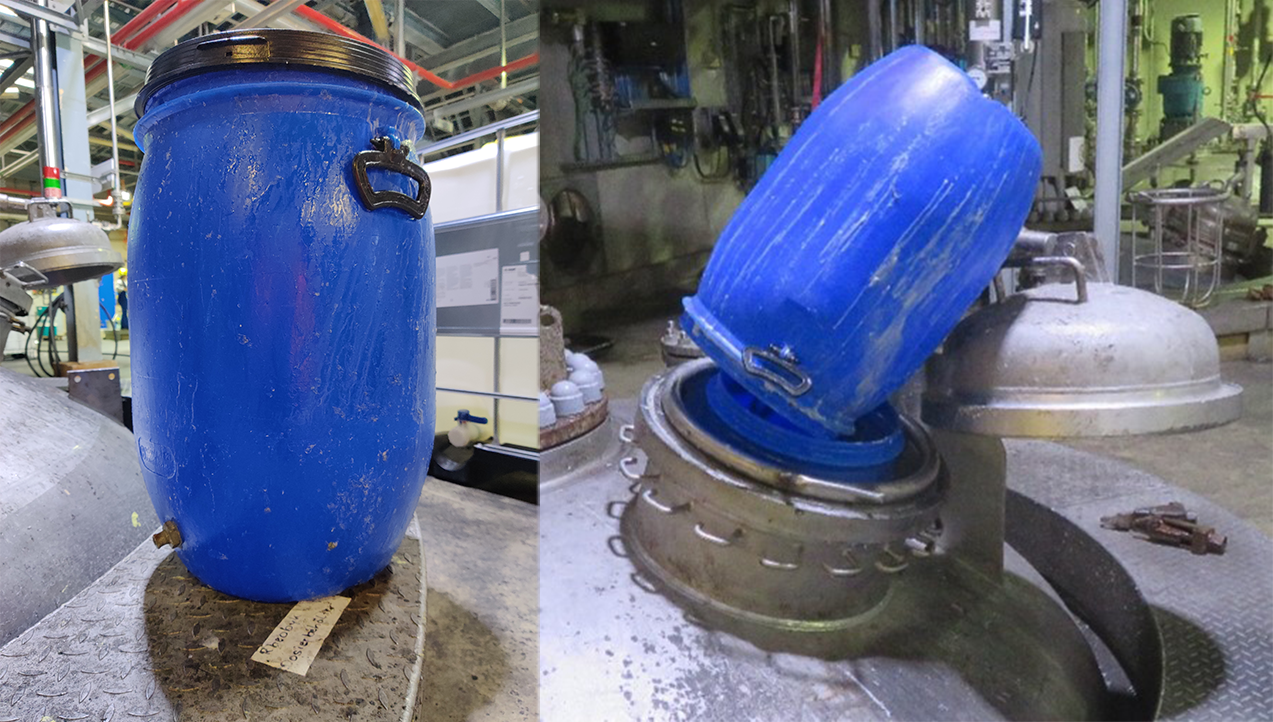
\includegraphics[width=0.5\textwidth]{img/dosierfass}
	\caption{Fotografien des Dosier- und des Transportfasses}
	\label{fig:dosierfass}
\end{figure}
\FloatBarrier
%Ende

\subsubsection{Soll-Zustand: Anforderung an die Dosierung}
Die Anforderungen an eine automatisierte Dosierung gliedern sich in mehrere Interessensgruppen auf. Beginnend mit der \textit{Technik}, sollen unter diesem Begriff jegliche Anforderungen der Prozess- und Sicherheitstechnik beschrieben sein. Beispielsweise fallen darunter die Dosierrate, die Dosiergenauigkeit und der zu beachtende Ex-Schutz. Die zweite Gruppierung beschreibt die Anforderungen der \textit{Produktion}, sprich die Interessen der auszuführenden Chemiefacharbeiter in der Anlage. Eine Forderung stellt dabei die einfache Bedienbarkeit dar. Zuletzt soll jedoch auch die \textit{Wartung} entsprechend leichtgängig und der Verschleiß des Dosiersystems gering sein. Die Forderungen aus den verschiedenen Perspektiven sind in Tabelle \ref{tab:anforderungen} zusammenfasst und wurden durch erfragen des Personals ermittelt und durch vorgegebenen Prozessparametern festgelegt.

% Table generated by Excel2LaTeX from sheet 'Daten'
\begin{table}[h!]
	\renewcommand*{\arraystretch}{1.2}
	\centering
	\caption{Anforderungen an die Verdickungsmittel-Dosierung}
	\label{tab:anforderungen}
	\resizebox{\textwidth}{!}{
		\begin{tabulary}{1.2\textwidth}{LL|L|L}
			\hline
			\multicolumn{2}{l|}{\textbf{Technik}} & \textbf{Produktion} & \textbf{Wartung}\\
			\hline
			Dosierrate: & 22 bis \SI{44}{\kilo \gram \per \hour}&einfache Bedienbarkeit&geringer Verschleiß\\
			Dosiergenauigkeit: & $\pm \, \SI{200}{\gram}$	& leichte Reinigung & leichte Wartung\\
			Ex-Schutz:	 & Zone 2 &Zeitersparnis&\\
			Risiko:  &minimal&&\\
			Verdickungsmittel: &TAFIGEL PUR 85&&\\
			Prozessleitsystem: &im PLS einsehbar&&\\
			Adaptierbarkeit:& für weitere Tanks adaptierbar &&\\
			Aufstellungsort: &siehe Abbildung \ref{fig:aufstellungsort}&&\\
			Einleitung: &siehe Abbildung \ref{fig:flansch}&&\\
			\hline
	\end{tabulary}}
\end{table}%
\FloatBarrier

Da weder die geforderte Dosiergenauigkeit erfasst, noch der Dosierstrom in der aktuellen Dosierung gemessen wird, ist eine signifikante Differenz zwischen Ist- und Soll-Anforderung an die Dosierung aus Perspektive der Technik erfüllt und das Dosierproblem somit als solches verifiziert. Die Perspektive der Produktion unterstützt diese Verifikation, da Anforderungen aufgrund der benötigten Vorbereitungszeit und der Sauberkeit der Dosierprozesses derzeit nicht erfüllt werden. Aus Sicht der Wartung besteht kein Handlungsbedarf.

\begin{figure}[h!]
	\begin{minipage}[b]{0.4\textwidth}
		\centering
		\includegraphics[height=4.25cm]{img/aufstellungsort}
		\caption{Ort für Dosierung}
		\label{fig:aufstellungsort}
	\end{minipage}
	%\hspace*{0.05\textwidth}
	\begin{minipage}[b]{0.55\textwidth}
		\centering
		\includegraphics[height=4.25cm]{img/flansch}
		\caption{Flansch für eingehenden Dosierstrom}
		\label{fig:flansch}
	\end{minipage}
\end{figure}
\FloatBarrier

%geringer Verschleiß
%leichte Wartung
%einfach zu Bedienen
%leichte Reinigung --> Spülbarkeit
%Dosiergenauigkeit und DOsierstrom
%--> SAmmeln von Informationen im Werk
% Platz im Werk mit Geometrie
%
%Kampagne
%Mitarbeiterkosten sparen
%Zeitersparnis
%Einfachheit
%Ex-Schutz
%PLS
%Prozesssicherheit

\subsubsection{Ergebnisse der experimentellen Untersuchungen}
\label{sec:analyse}
In der zu planenden Dosierung soll auf das Verdickungsmittel TAFIGEL PUR 85 der \mbox{\textsc{Münzing Chemie Gmbh}} zurückgegriffen werden. Laut Hersteller handelt es sich hierbei um einen assoziativen Polyurethan-Verdicker, welcher durch Gerüstbildung zwischen Verdickermolekülen, Bindemittel und Pigmentpartikeln die gewünschte Viskosität hervorruft und stabilisiert. Diese Beschreibung deckt sich mit der unter Abschnitt \ref{sec:grundlagen} formulierten Beschreibung der Assoziativverdicker. \cite{MunzingChemieGmbH.2014}
%--> Datenblätter
Die Ergebnisse der Viskositätsmessungen gliedern sich nach der Durchführung in Abschnitt \ref{sec:durchführung} in die Verifizierung der angegebenen Viskosität, der Untersuchung der Temperaturabhängigkeit, der Untersuchung der Verdünnungsabhängigkeit und in Pumpversuche.
Beginnend mit der Verifizierung der angegeben Viskosität sind in Abbildung \ref{dia:visko} die gemessenen Viskositäten des TAFIGEL PUR 85 und des Rheobyk-H 3300 VF dargestellt. 

%START DIAGRAMM

\begin{figure}[h]
	\begin{center}
		%\resizebox{\textwidth}{!}{
		\begin{tikzpicture}
			\begin{axis}[
				grid=both,
				grid style={line width=.1pt, draw=gray!10},
				major grid style={line width=.2pt,draw=gray!50},
				width= 0.95 \textwidth,
				height=0.5\textwidth,
				symbolic x coords={, Messreihe 1, Messreihe 2, Messreihe 3, Messreihe 4, Messreihe 5, \shortstack[c]{\SI{50}{\milli \liter} \\ Becherglas},},
				axis y line = left,
				axis x line = bottom,
				xtick=data,
				ytick={0,5,...,65},
				ymax = 65,
				ymin=0,
				ylabel=dynamische Viskosität in \si{\pascal \second},
				legend style={at={(0.475,1.05)},anchor=west},
				legend cell align={left}]
				%Tafigel
				\addplot[color=black,mark=*, only marks] coordinates {
					(Messreihe 1, 49.080)
					(Messreihe 2, 50.760)
					(Messreihe 3, 52.000)
					(Messreihe 4, 53.000)
					(Messreihe 5, 51.600)
					(\shortstack[c]{\SI{50}{\milli \liter} \\ Becherglas}, 50.87)
				};
				\addplot[color=black,dashed] coordinates {
				(Messreihe 1, 51.21)
				(\shortstack[c]{\SI{50}{\milli \liter} \\ Becherglas}, 51.21)
				};
				%Rheobyk
				\addplot[color=black,mark=o, only marks] coordinates {
					(Messreihe 1, 24.000)
					(Messreihe 2, 24.800)
					(Messreihe 3, 22.880)
					(Messreihe 4, 23.890)
					(Messreihe 5, 24.200)
					(\shortstack[c]{\SI{50}{\milli \liter} \\ Becherglas}, 23.32)
				};
				\addplot[color=black,dotted] coordinates {
					(Messreihe 1, 23.85)
					(\shortstack[c]{\SI{50}{\milli \liter} \\ Becherglas}, 23.85)
				};
			\legend{TAFIGEL PUR 85, Mittelwert (\SI{51}{\pascal \second}), Rheobyk-H 3300 VF, Mittelwert (\SI{24}{\pascal \second}) };
			\end{axis}
		\end{tikzpicture}
		%}
		\caption{Dynamische Viskositäten der Verdickungsmittel TAFIGEL PUR 85 und Rheobyk-H 3300 VF}
		\label{dia:visko}
	\end{center}
\end{figure} 

\FloatBarrier 
%ENDE

Die sich aus den Messwerten ergebenden Mittelwerte ergeben eine Viskosität für TAFIGEL PUR 85 mit \SI{51}{\pascal \second} und für Rheobyk-H 3300 VF \SI{24}{\pascal \second}. Zum Vergleich: Die Viskosität des TAFIGEL PUR 85 ist im Sicherheitsdatenblatt unter  \cite{MunzingChemieGmbH.2020} mit rund \SI{35}{\pascal \second}  angegeben. Auf Nachfrage beim Hersteller ist diese Schwankung produktionsbedingt und beeinträchtigt die Wirksamkeit des Verdickungsmittels nicht. Ebenfalls zu erkennen ist, dass die Messwerte Abweichungen vom Mittelwert aufzeigen. Statistisch ergeben sich daraus relativen Standardabweichungen für die Messwerte des TAFIGEL PUR\,85 mit \SI{2,4}{\percent} und für das Rheobyk-H 3300 VF mit \SI{2,6}{\percent}. Die Messungen im \SI{50}{\milli \liter}, statt im \SI{600}{\milli \liter} Becherglas zeigten keine maßgeblichen Unterscheide.\linebreak
%--> nach DIN
%--> beide Verdickungsmittel
Eine weitere Untersuchung beschäftigte sich mit der Temperaturabhängigkeit des Verdickungsmittels. Dafür wurde zum einen der Verlauf der Dichte in Abhängigkeit von der Temperatur für das TAFIGEL PUR 85 bei der \textsc{Münzing Chemie GmbH} angefragt. Die erhaltenen Daten sind in Abbildung \ref{dia:dichte} zu sehen.

%START DIAGRAMM

\begin{figure}[h]
	\begin{center}
		%\resizebox{\textwidth}{!}{
			\begin{tikzpicture}
				\begin{axis}[
					grid=both,
					grid style={line width=.1pt, draw=gray!10},
					major grid style={line width=.2pt,draw=gray!50},
					width= 0.95 \textwidth,
					height=0.33\textwidth,
					%symbolic x coords={, Messreihe 1, Messreihe 2, Messreihe 3, Messreihe 4, Messreihe 5, \shortstack[c]{\SI{50}{\milli \liter} \\ Becherglas},},
					axis y line = left,
					axis x line = bottom,
					xtick={0,5,...,50},
					ytick={950,975,...,1050},
					xmax=50,
					ymax = 1050,
					ymin=950,
					xmin=0,
					ylabel=Dichte in \si{\kilo \gram \per \kmeter},
					xlabel = Temperatur in \si{\celsius},
					legend style={at={(1.0,0.95)},anchor=east},
					legend cell align={left},
					ylabel style={yshift=0.4cm},]
					%Tafigel
					\addplot[color=black,mark=*, only marks] coordinates {
						(10, 1034)
						(20, 1010)
						(30, 1008)
						(40, 1001)
					};				
					\legend{TAFIGEL PUR 85};
				\end{axis}
			\end{tikzpicture}
			%}
		\caption{Dichte des TAFIGEL PUR 85 in Abhängigkeit von der Temperatur}
		\label{dia:dichte}
	\end{center}
\end{figure} 

\FloatBarrier 
%ENDE

Zu erkennen ist, dass sich die Dichte im Bereich zwischen 10 und \SI{40}{\celsius} mit steigender Temperatur verringert. Der Verlauf und der Umfang der Daten lässt nicht eindeutig auf einen linearen Zusammenhang zwischen Dichte und Temperatur schließen, jedoch ist erkennbar, dass ein signifikanter Unterschied in der Dichte für 10 und für \SI{40}{\celsius} besteht. Im Bereich zwischen 20 und \SI{30}{\celsius} bleibt die Dichte hingegen konstant. Aus den Daten wurde ermittelt, dass zwischen den Messungen eine relative Standardabweichung von \SI{1,4}{\percent} vorliegt.\linebreak
Neben dem Erfragen des Zusammenhangs zwischen Dichte und Temperatur ist auch die Abhängigkeit der Viskosität von der Temperatur untersucht worden. Der Grund hierfür liegt in der zuvor bestimmten Viskosität des Verdickungsmittels bei rund \SI{50}{\pascal \second}. Da im Regelfall bei der \textsc{Alberdingk Boley Leuna GmbH} keine so hohen Viskositäten gefördert werden, bot sich die Überlegung an die Viskosität durch Wärmezufuhr zu reduzieren. Das Ergebnis der dafür genutzten Versuchsreihe ist in Abbildung \ref{dia:temp} zu finden. Darin lässt sich erkennen, dass der Zusammenhang zwischen Viskosität und Dichte in diesem Temperaturbereich eine Linearität mit einem Bestimmtheitsmaß von \SI{99,6}{\percent} aufweist. Mit steigender Temperatur sinkt dabei die Viskosität. Der negative Anstieg lässt zudem darauf deuten, dass bei einer Temperaturerhöhung um \SI{5}{\kelvin} eine Verringerung der Viskosität um \SI{10}{\pascal \second} stattfindet.

%START DIAGRAMM

\begin{figure}[h]
	\begin{center}
		%\resizebox{\textwidth}{!}{
			\begin{tikzpicture}
				\begin{axis}[
					grid=both,
					grid style={line width=.1pt, draw=gray!10},
					major grid style={line width=.2pt,draw=gray!50},
					width= 0.95 \textwidth,
					height=0.4\textwidth,
					%symbolic x coords={, Messreihe 1, Messreihe 2, Messreihe 3, Messreihe 4, Messreihe 5, \shortstack[c]{\SI{50}{\milli \liter} \\ Becherglas},},
					axis y line = left,
					axis x line = bottom,
					xtick={0,5,...,50},
					ytick={0,5,...,65},
					xmax=50,
					ymax = 65,
					ymin=0,
					xmin=0,
					ylabel=dynamische Viskosität in \si{\pascal \second},
					xlabel = Temperatur in \si{\celsius},
					legend style={at={(1.,1.125)},anchor=east},
					legend cell align={left},
					%ylabel style={yshift=0.4cm},
					]
					%Tafigel
					\addplot[color=black,mark=*, only marks] coordinates {
						(21, 50.1)
						(25, 39.5)
						(30, 30.2)
						(35, 19.2)
						(39, 12.6)
					};
				
				\addplot [domain = 0:50, dashed] {-2.07*x+92.26};
							
					\legend{TAFIGEL PUR 85,$\eta(\vartheta) = -\SI{2,07}{\pascal \second \per \celsius}*\vartheta+\SI{92,26}{\pascal\second} \, | \, R^2 = \SI{99,6}{\percent}$};
				\end{axis}
			\end{tikzpicture}
			%}
		\caption{Dynamische Viskosität des TAFIGEL PUR 85 in Abhängigkeit von der Temperatur}
		\label{dia:temp}
	\end{center}
\end{figure} 
\FloatBarrier 
%ENDE
Zusätzlich wurde neben dem Aspekt der Erwärmung des Verdickungsmittels wurde auch der Effekt der Verdünnung auf die Viskosität untersucht. Es wird erwartet, dass mit sinkender Konzentration an Verdickungsmittel die Viskosität des Verdickungsmittels ebenfalls sinkt. In Abbildung \ref{dia:verdunnung} sind die Messergebnisse der Viskositäten beider Verdickungsmittel TAFIGEL PUR 85 und Rheobyk-H 3300 VF dargestellt. In separaten x-Achsen sind der Anteil an Verdickungsmittel und der Anteil an reiner Aktivsubstanz der Verdickungsmittels aufgetragen.

%START DIAGRAMM

\begin{figure}[h]
	\begin{center}
		%\resizebox{\textwidth}{!}{
			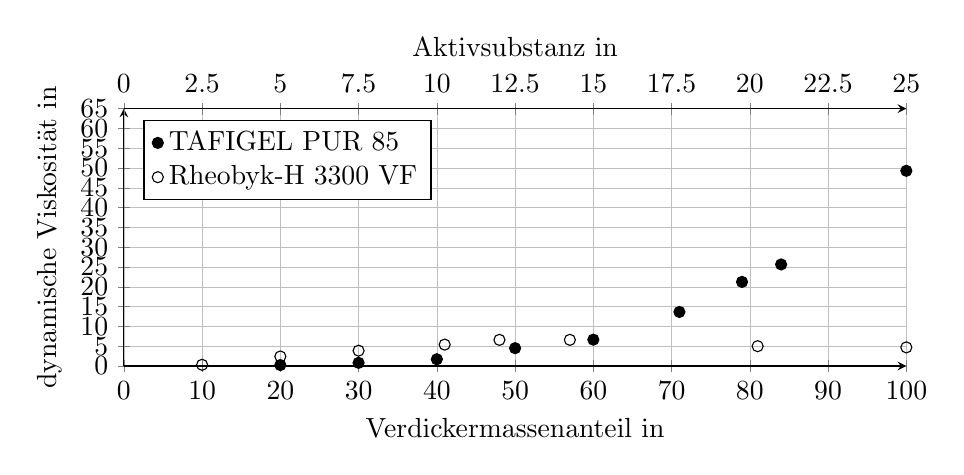
\begin{tikzpicture}
				\begin{axis}[
					grid=both,
					grid style={line width=.1pt, draw=gray!10},
					major grid style={line width=.2pt,draw=gray!50},
					width= 0.95 \textwidth,
					height=0.4\textwidth,
					%symbolic x coords={, Messreihe 1, Messreihe 2, Messreihe 3, Messreihe 4, Messreihe 5, \shortstack[c]{\SI{50}{\milli \liter} \\ Becherglas},},
					axis y line = left,
					axis x line = bottom,
					xtick={0,10,...,100},
					ytick={0,5,...,65},
					xmax=100,
					ymax = 65,
					ymin=0,
					xmin=0,
					ylabel=dynamische Viskosität in \si{\pascal \second},
					xlabel = Verdickermassenanteil in \si{\mpercent},
					legend style={at={(0.025,0.8)},anchor=west},
					legend cell align={left},
					%ylabel style={yshift=0.4cm},
					]
					%Tafigel
					\addplot[color=black,mark=*, only marks] coordinates {
						(20, .230)
						(30, .800)
						(40, 1.700)
						(50, 4.500)
						(60, 6.650)
						(71, 13.650)
						(79, 21.240)
						(84, 25.650)
						(100, 49.300)
					};
				%Rheobyk
				\addplot[color=black,mark=o, only marks] coordinates {
					(10, 0.300)
					(20, 2.400)
					(30, 3.870)
					(41, 5.400)
					(48, 6.600)
					(57, 6.600)
					(81, 5.000)
					(100, 4.700)
	
				};
					\legend{TAFIGEL PUR 85, Rheobyk-H 3300 VF};
				\end{axis}
			\begin{axis}[
				width= 0.95 \textwidth,
				height=0.4\textwidth,
				%symbolic x coords={, Messreihe 1, Messreihe 2, Messreihe 3, Messreihe 4, Messreihe 5, \shortstack[c]{\SI{50}{\milli \liter} \\ Becherglas},},
				hide y axis,
				axis x line = top,
				xtick={0,2.5,...,25},
				xmax=25,
				xmin=0,
				xlabel = Aktivsubstanz in \si{\mpercent},
				legend style={at={(1.,1.125)},anchor=east},
				legend cell align={left},
				]
				%Tafigel
				\addplot[draw=none, forget plot] coordinates {
					(5, .230)
					(7.5, .800)
					(10, 1.700)
					(12.5, 4.500)
					(15, 6.650)
					(17.7, 13.650)
					(19.9, 21.240)
					(20.9, 25.650)
					(25, 49.300)
				};
			\end{axis}
			\end{tikzpicture}
			%}
		\caption{Dynamische Viskositäten der Verdickungsmittel  TAFIGEL PUR 85 und Rheobyk-H 3300 VF in Abhängigkeit vom Massenanteil des Verdickungsmittels bzw. dem Anteil an Aktivsubstanz}
		\label{dia:verdunnung}
	\end{center}
\end{figure} 
\FloatBarrier 
%ENDE
Durch dieses Diagramm zeigt sich, dass sich beide Verdickungsmittel in ihrem Verdünnungsverhalten deutlich unterscheiden. Während das Rheobyk-H 3300 VF ab \SI{40}{\mpercent} eine vergleichsweise stabile Viskosität in Abhängigkeit von der Verdünnung aufzeigt, lässt sich für das TAFIGEL PUR 85 eine starke Abhängigkeit zwischen Viskosität und Verdickermassenanteil festzustellen. Auffallend ist zudem, dass die Viskosität des Rheobyk-H 3300 VF im Bereich zwischen 50 und \SI{60}{\mpercent} höher ist als mit einem Verdickeranteil von \SI{100}{\mpercent}.\linebreak
%
%\subsubsection{Verdünnungsverhalten}
%%--> Eigenregie
%
%\subsubsection{Erwärmungsverhalten}
%%--> beim Hersteller angefragt
%

Um die Lagerungsfähigkeit des TAFIGEL PUR 85 zu überprüfen wurde vom 08.11.2021 bis zum 08.12.2021 eine vierteilige Bilderreihe aufgenommen, um eine mögliche Sedimentation des emulgierten Polymers im Verdickungsmittel festzustellen. Diese Bilderreihe ist Abbildung \ref{fig:lagerung} zu sehen und die abgelesenen Volumina in Tabelle \ref{tab:lagerung} zusammengefasst.

%\begin{figure}[h!]
%	\centering
%	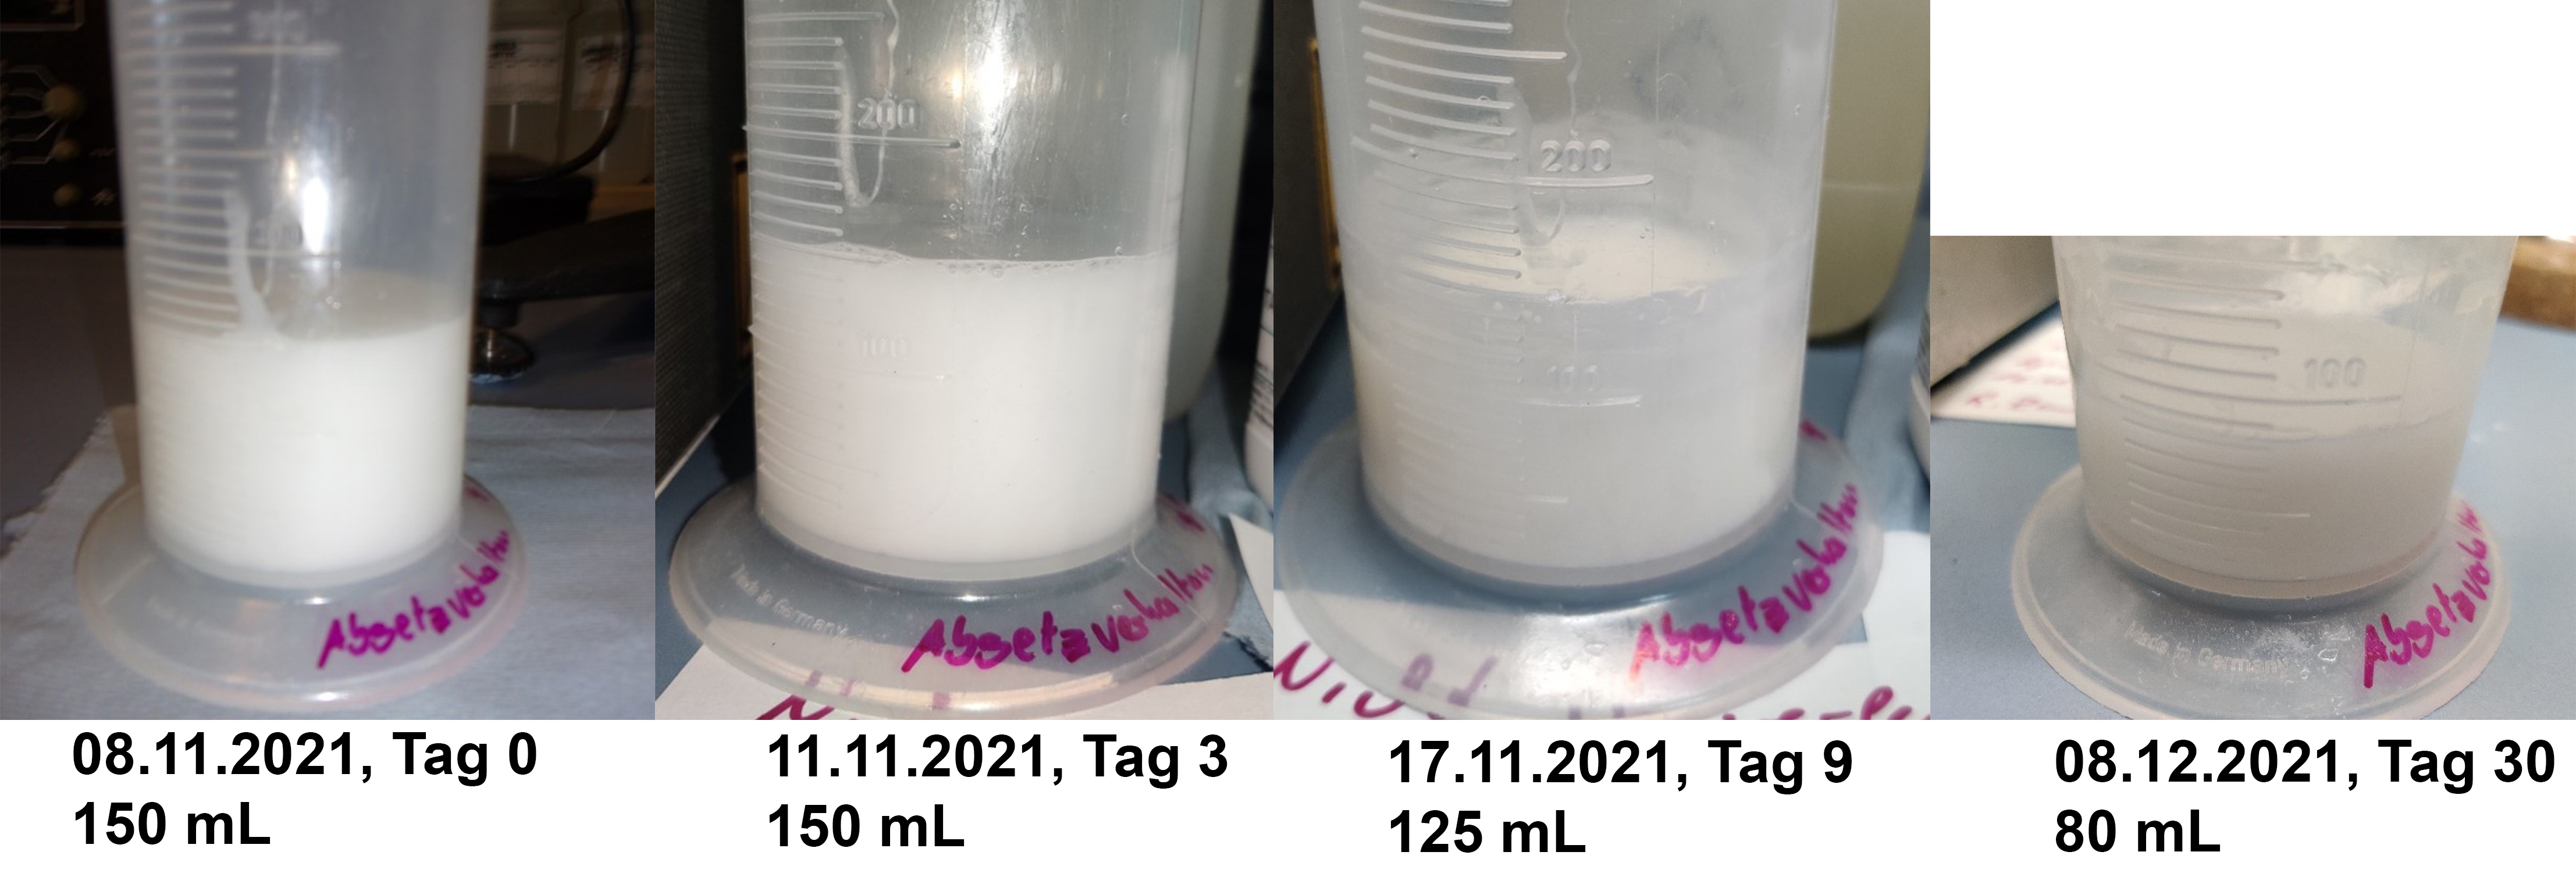
\includegraphics[width=0.75\textwidth]{img/lagerung}
%	\caption{Fotografien der offenen Lagerung des TAFIGEL PUR 85}
%	\label{fig:lagerung}
%\end{figure}
%\FloatBarrier
%%Ende

\begin{figure}[h!]
	\begin{minipage}[b]{0.55\textwidth}
		\centering
		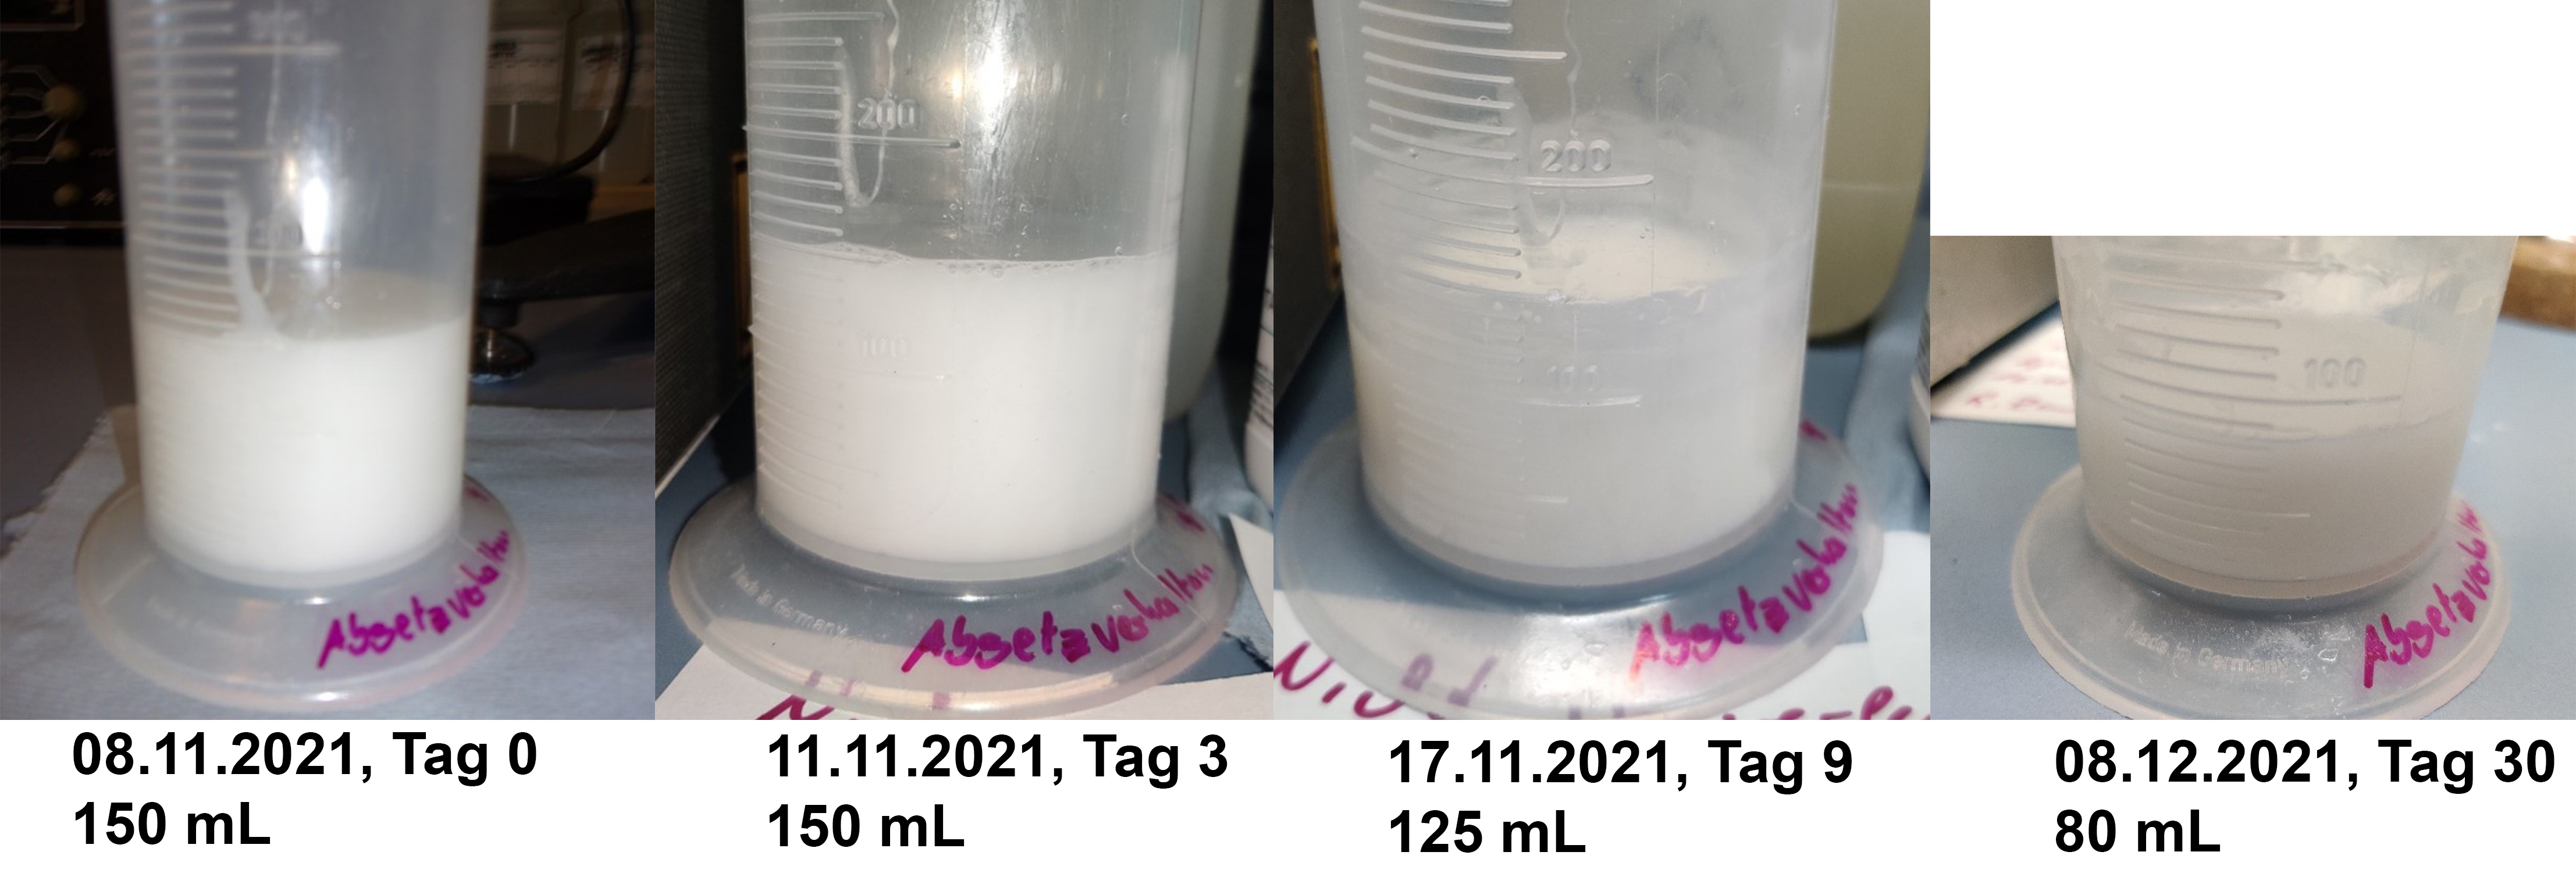
\includegraphics[width=1.1\textwidth]{img/lagerung}
		\caption{Fotografien der offenen Lagerung}
		\label{fig:lagerung}
	\end{minipage}
	%\hspace*{0.05\textwidth}
	\begin{minipage}[b]{0.42\textwidth}
		\centering
		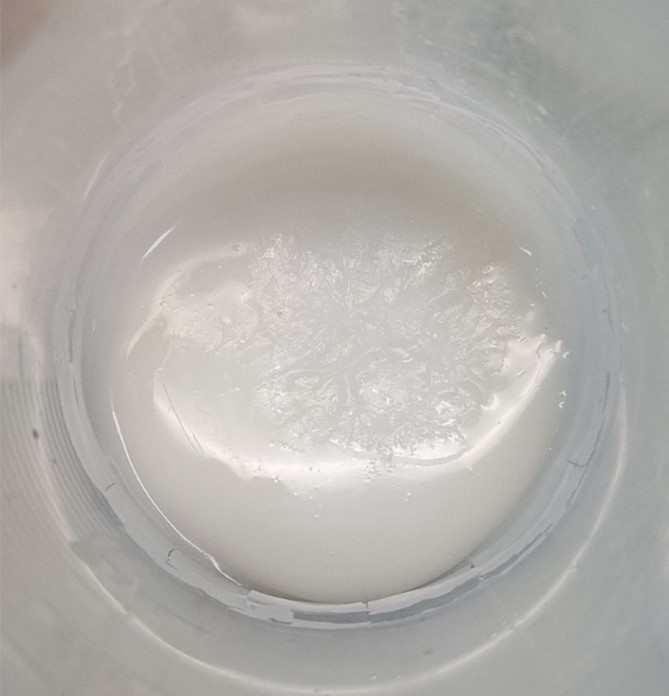
\includegraphics[width=0.5\textwidth]{img/rahmschicht}
		\caption{Fotografie der Rahmschicht}
		\label{fig:rahmschicht}
	\end{minipage}
\end{figure}
\FloatBarrier

In der Bildern des Versuches ist die Volumenabnahme des Verdickungsmittels über die Zeit festzustellen. Das Bild am Tag 9 zeigt, dass das Polymer des Verdickungsmittels zum Teil an der Zylinderwand haften bleibt. Im Verlauf der Zeit verändert sich das anhaftende Polymer von einem milchigen-weißen zu einer durchsichtigen Schicht, welche am Tag 30 noch durch Schlieren erkennbar sind. Des weiteren ist ab der Beobachtung an Tag 9 auch die Bildung einer "`Rahmschicht"' zu beobachten, welche auch in \cite{MunzingChemieGmbH.2014} beschrieben ist (vgl. Abbildung \ref{fig:rahmschicht}). Der Hersteller rät für diese Beobachtung in \cite{MunzingChemieGmbH.2014} zum Aufrühren des Verdickungsmittel vor der Nutzung. Derartige Veränderungen sind bei geschlossener Lagerung des TAFIGEL PUR 85  nicht zu erkennen.

% Table generated by Excel2LaTeX from sheet 'Daten'
\begin{table}[h!]
	\renewcommand*{\arraystretch}{1.2}
	\centering
	\caption{Volumina des Verdickungsmittels bei offener Lagerung}
	\label{tab:lagerung}
%	\resizebox{10.5cm}{!}{
		\begin{tabulary}{1.0\textwidth}{L|C|C|C|C}
			\hline
			\textbf{Datum} & 08.11.2021 & 11.11.2021 & 17.11.2021 & 08.12.2021\\
			\hline
			\textbf{Tag}&0&3&9&30\\
			\hline
			\textbf{Volumen $\left[\si{\milli \liter}\right]$}&150&150&125&80\\
			\hline			
	\end{tabulary}
%}
\end{table}%
\FloatBarrier

%\begin{figure}[h!]
%	\centering
%	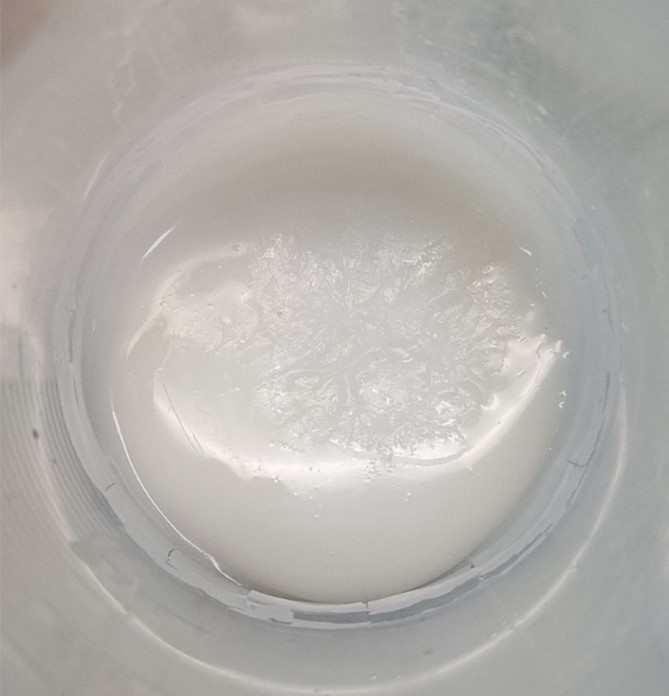
\includegraphics[width=0.15\textwidth]{img/rahmschicht}
%	\caption{Rahmschicht bei offener Lagerung des TAFIGEL PUR 85}
%	\label{fig:rahmschicht}
%\end{figure}
%\FloatBarrier
%%Ende

Die im Zylinder übriggebliebenen \SI{80}{\milli \liter} des TAFIGEL PUR 85 sind anschließend mit einer nicht definierten Wassermenge verdünnt und eine Viskosität von rund \SI{3000}{\milli \pascal \second} bestimmt worden. Zusätzlich wurde mittels Trockenschrank und Waage ein Feststoffgehalt von \SI{11}{\mpercent} ermittelt und die Ergebnisse mit Abbildung \ref{dia:verdunnung} verglichen und ließen sich verifizieren. Daraus ließ sich ebenfalls Ablesen, dass die angemischte Probe einem Verdickungsmittelanteil von ca. \SI{44}{\mpercent} entspricht. Die optische Erscheinung der Probe am 08.12.2021 und am 08.02.2021 ist in Abbildung \ref{fig:lagerung2} aufgezeigt und wiesen keine makroskopischen Unterschiede auf.

\begin{figure}[h!]
	\centering
	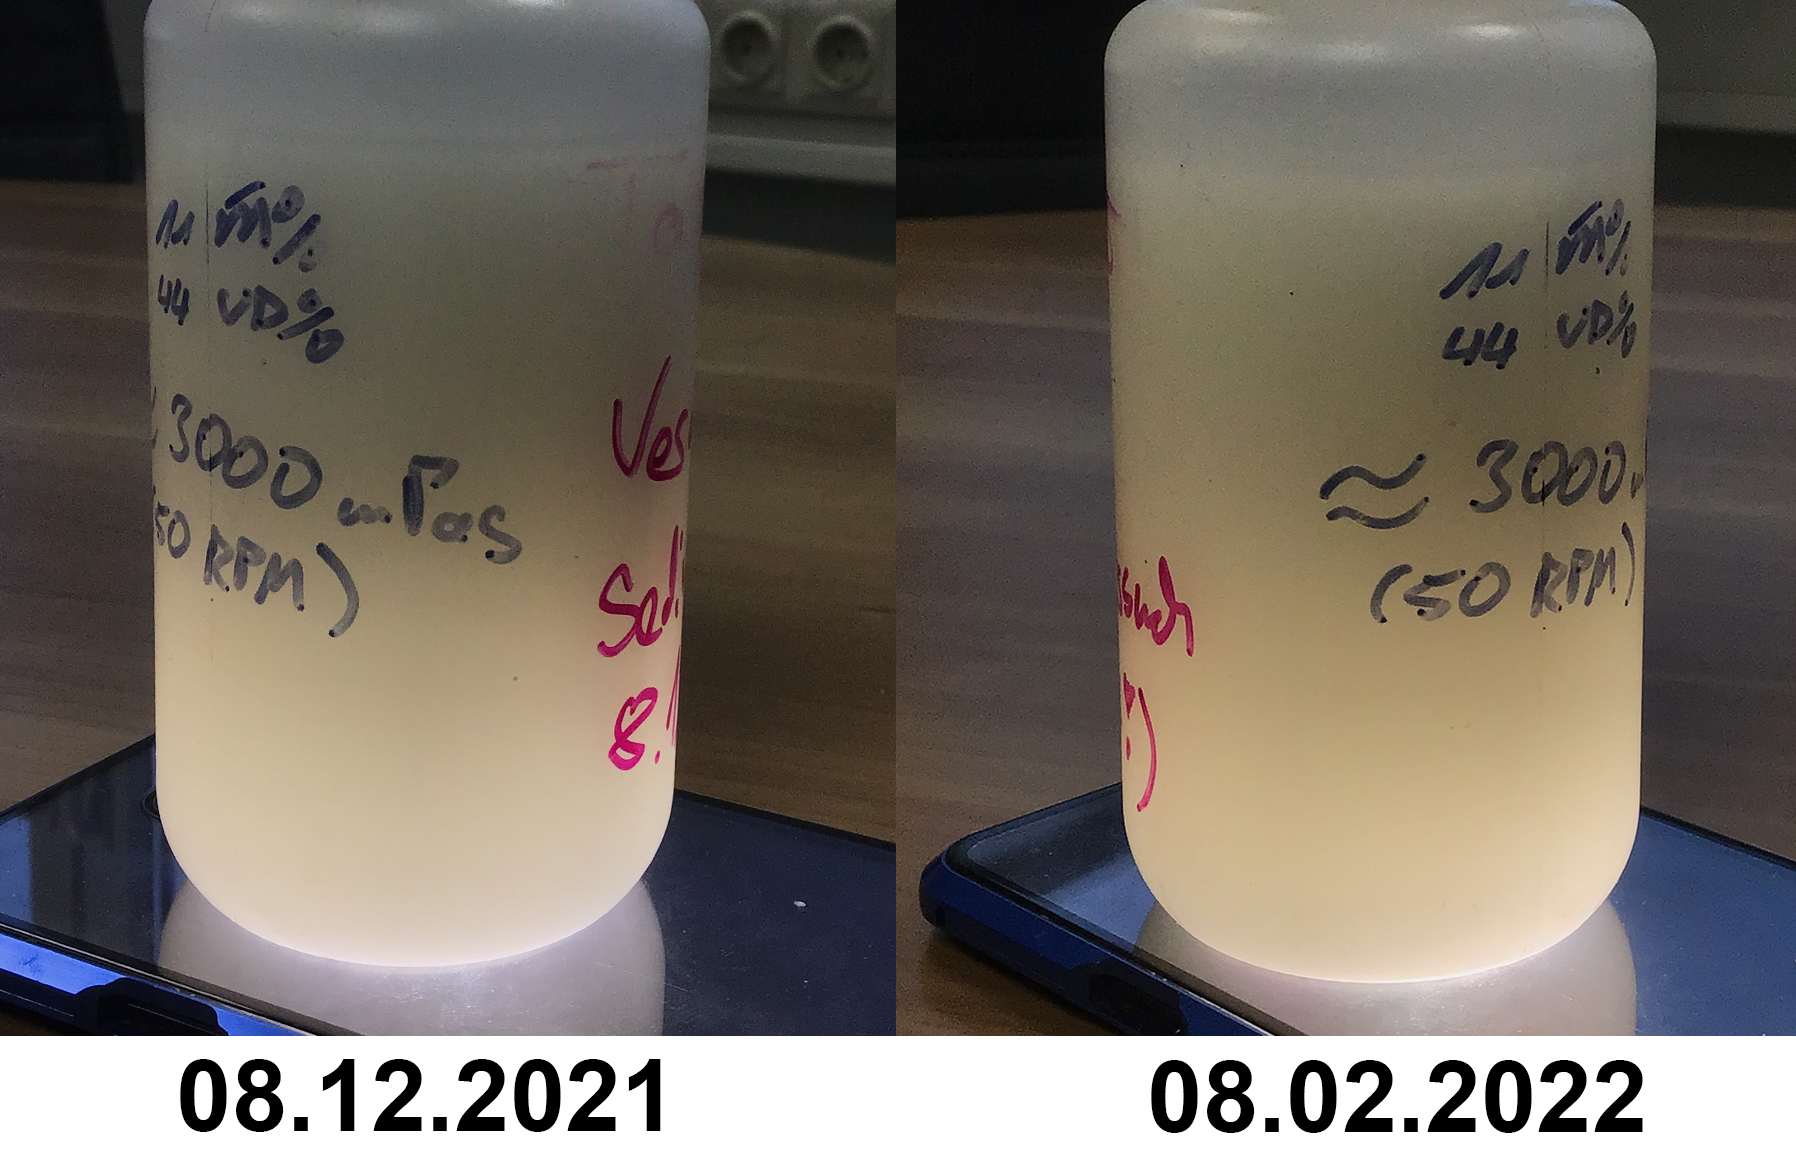
\includegraphics[width=0.5\textwidth]{img/lagerung2}
	\caption{Makroskopischer Vergleich des verdünnten TAFIGEL PUR 85}
	\label{fig:lagerung2}
\end{figure}
\FloatBarrier
%Ende

Im Laufe der Überlegungen zur Umsetzung der Dosierung wurde die Möglichkeit der Dosierung mit einer Pumpe in Betracht gezogen. Durch die hohe Viskosität und den Anforderungen an Sauberkeit und Wartung, sollte zunächst die Pumpbarkeit des TAFIGEL\,PUR\,85 mit einer Schlauchpumpe überprüft werden. Die Ergebnisse der Massenströme bei verschiedenen Drehzahlen ist im Diagramm unter Abbildung \ref{dia:pumpe} gezeigt. Zum Vergleich ist ebenfalls Pumpenkennlinie bei der Förderung Wasser mit einer Temperatur von \SI{20}{\celsius} und einem Druck von \SI{2}{\bar} dargestellt. Diese bestimmte sich aus der vom Hersteller angegebenen Kennlinie für den Volumenstrom in \cite{PonndorfGeratetechnikGmbH.2020}.

\begin{figure}[h]
	\begin{center}
		%\resizebox{\textwidth}{!}{
			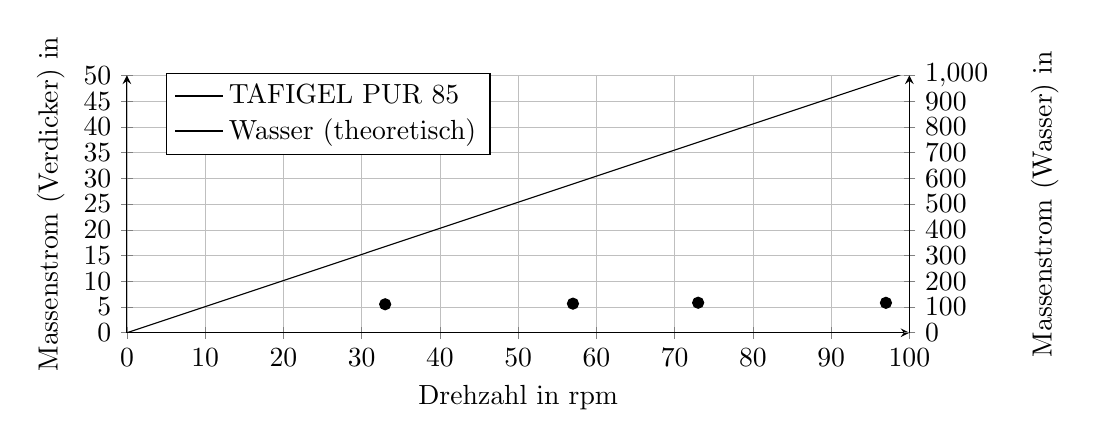
\begin{tikzpicture}
				\begin{axis}[
					grid=both,
					grid style={line width=.1pt, draw=gray!10},
					major grid style={line width=.2pt,draw=gray!50},
					width= 0.95 \textwidth,
					height=0.4\textwidth,
					%symbolic x coords={, Messreihe 1, Messreihe 2, Messreihe 3, Messreihe 4, Messreihe 5, \shortstack[c]{\SI{50}{\milli \liter} \\ Becherglas},},
					axis y line = left,
					axis x line = bottom,
					xtick={0,10,...,100},
					ytick={0,5,...,50},
					xmax=100,
					ymax = 50,
					ymin=0,
					xmin=0,
					ylabel= Massenstrom (Verdicker) in \si{\kilo \gram \per \hour},
					xlabel = Drehzahl in \si{rpm},
					legend style={at={(1.0,0.9)},anchor=east},
					legend cell align={left},
					]
					%Tafigel
					\addplot[color=black,mark=*, only marks] coordinates {
						(33, 5.53)
						(57, 5.65)
						(73, 5.83)
						(97, 5.81)
					};	\label{tafigel}
%					%Wasser
%					\addplot[color=black,no markers, domain=0:100] {10.14*x+0};			
					%\legend{Massenstrom - TAFIGEL PUR 85};
				\end{axis}
			\begin{axis}[
				width= 0.95 \textwidth,
				height=0.4\textwidth,
				%symbolic x coords={, Messreihe 1, Messreihe 2, Messreihe 3, Messreihe 4, Messreihe 5, \shortstack[c]{\SI{50}{\milli \liter} \\ Becherglas},},
				axis y line = right,
				hide x axis,
				xtick={0,10,...,100},
				ytick={0,100,...,1000},
				ymax=1000,
				ymin=0,
				xmin=0,
				xmax=100,
				ylabel= Massenstrom (Wasser) in \si{\kilo \gram \per \hour},
				xlabel = Drehzahl in \si{rpm},
				legend style={at={(0.05,0.85)},anchor=west},
				legend cell align={left},
				ylabel style={yshift=-0.3cm},
				]	
				\addlegendimage{/pgfplots/refstyle=tafigel}\addlegendentry{TAFIGEL PUR 85}
				%Wasser
				\addplot[color=black,no markers, domain=0:100] {10.14*x+0};			
				\addlegendentry{Wasser (theoretisch)};
			\end{axis}
			\end{tikzpicture}
			%}
		\caption{Massenstrom in Abhängigkeit von der Drehzahl für TAFIGEL PUR 85 und Wasser mit einer \textsc{Ponndorf P Classic 25} Schlauchpumpe}
		\label{dia:pumpe}
	\end{center}
\end{figure} 

\FloatBarrier 
%ENDE

Im Diagramm ist zu sehen, dass der Verlauf des theoretisch geförderten Massenstrom an Wasser linear zur Drehzahl steigt. Im Vergleich dazu zeigt sich der gemessene Förderstrom des Verdickungsmittels unabhängig von der Drehzahl konstant bei ca. 5 bis \SI{6}{\kilo \gram \per \hour}. Es wäre zu erwarten gewesen, dass für das Verdickungsmittel ähnlich wie bei der Kennlinie für Wasser mit steigender Drehzahl der Massenstrom steigt. Zusätzlich dazu sind die Dimensionen der Förderströme zwischen Wasser und Verdickungsmittel komplett unterschiedlich. Dies ist unter anderem an den verschiedenen Skalen der beiden y-Achsen zu erkennen.\linebreak
Da die getestete Pumpe zunächst nur zum Testen der Pumpfähigkeit genutzt wurde, sind weitere Auswertungen zum volumetrischen Wirkungsgrad erfolgt. Da keine Daten bezüglich dieses Fluids bei dieser Schlauchpumpe vorliegen, wird zunächst aufgrund der großen Viskositätsunterschiede zwischen Wasser und TAFIGEL PUR 85 angenommen, dass das Verdrängungsvolumen der Förderung von Wasser einem volumetrischen Wirkungsgrad von \SI{100}{\percent} entspricht. \linebreak
Die Berechnung des volumetrischen Wirkungsgrades erfolgt gemäß Gleichung \eqref{eq:vol_wirkungsgrad}, wobei der theoretische Volumenstrom dem vom Hersteller angegebenen Volumenstrom für Wasser bei \SI{2}{\bar} entspricht. In Gleichung \eqref{gl:vol_wirkungsgrad} ist ein Beispiel für eine solche Berechnung dargestellt und die Ergebnisse sind in Tabelle \ref{tab:wirkungsgrad}  und Abbildung \ref{dia:wirkungsgrad} zusammengefasst und veranschaulicht.

\begin{flalign}
	\label{gl:vol_wirkungsgrad}
	\eta_V &= \frac{\dot{V}}{\dot{V}_{\text{theo}}} = \frac{\dot{V}_{\text{VD}}}{\dot{V}_{\text{\ce{H2O}}}} = \frac{\dot{m}_{\text{VD}}*\rho_{\text{\ce{H2O}}}}{\dot{m}_{\text{\ce{H2O}}}*\rho_{\text{VD}}} \\[2mm]
	\eta_V (\SI{33}{\rpm}) &= \frac{\SI{5,5}{\kg \per \hour}*\SI{1000}{\kg \per \kmeter}}{\SI{335}{\kg \per \hour}*\SI{1040}{\kg \per \kmeter}} = \underline{\SI{1,64}{\percent}}
\end{flalign}

% Table generated by Excel2LaTeX from sheet 'Daten'
\begin{table}[h!]
	\renewcommand*{\arraystretch}{1.2}
	\centering
	\caption{Ergebnisse der Berechnung des volumetrischen Wirkungsgrades für TAFIGEL PUR 85 in Bezug auf Wasser für eine \textsc{Ponndorf P CLassic 25}}
	\label{tab:wirkungsgrad}
	%\resizebox{\textwidth}{!}{
		\begin{tabulary}{1.\textwidth}{C|CC|CC|C}
			\hline
			$n \left[\si{\umdrehung\per \minute}\right]$ & $\dot{m}_{\text{VD}} \left[\si{\kg\per \hour}\right]$ & $\dot{m}_{\text{\ce{H2O}}} \left[\si{\kg\per \hour}\right]$ & $\rho_{\text{VD}} \left[\si{\kg\per \kmeter}\right]$& $\rho_{\text{\ce{H2O}}} \left[\si{\kg\per \kmeter}\right]$& $\eta_V \left[\si{\percent}\right]$\\
			\hline
			33	&	5,5&335&\multirow{4}{*}{1040}	&\multirow{4}{*}{1000}&1,64\\
			57	&	5,7&578&						&&0,99\\
			73	&	5,8&740&						&&0,78\\
			97 	&	5,8&984&						&&0,59\\
			\hline			
	\end{tabulary}
%}
\end{table}%
\FloatBarrier

\begin{figure}[h]
	\begin{center}
		%\resizebox{\textwidth}{!}{
			\begin{tikzpicture}
				\begin{axis}[
					grid=both,
					grid style={line width=.1pt, draw=gray!10},
					major grid style={line width=.2pt,draw=gray!50},
					width= 0.95 \textwidth,
					height=0.4\textwidth,
					%symbolic x coords={, Messreihe 1, Messreihe 2, Messreihe 3, Messreihe 4, Messreihe 5, \shortstack[c]{\SI{50}{\milli \liter} \\ Becherglas},},
					axis y line = left,
					axis x line = bottom,
					xtick={0,10,...,100},
					ytick={0,1,...,10},
					xmax=100,
					ymax = 10,
					ymin=0,
					xmin=0,
					ylabel= $\dot{m}_{\text{VD}}$ in \si{\kilo \gram \per \hour},
					xlabel = Drehzahl in \si{rpm},
					legend style={at={(1.0,0.9)},anchor=east},
					legend cell align={left},
					]
					%Tafigel
					\addplot[color=black,mark=*, only marks] coordinates {
						(33, 5.53)
						(57, 5.65)
						(73, 5.83)
						(97, 5.81)
					};	\label{tafigel}
					%					%Wasser
					%					\addplot[color=black,no markers, domain=0:100] {10.14*x+0};			
					%\legend{Massenstrom - TAFIGEL PUR 85};
				\end{axis}
				\begin{axis}[
					width= 0.95 \textwidth,
					height=0.4\textwidth,
					%symbolic x coords={, Messreihe 1, Messreihe 2, Messreihe 3, Messreihe 4, Messreihe 5, \shortstack[c]{\SI{50}{\milli \liter} \\ Becherglas},},
					axis y line = right,
					hide x axis,
					xtick={0,10,...,100},
					ytick={0,0.5,...,5},
					ymax=5,
					ymin=0,
					xmin=0,
					xmax=100,
					ylabel= $\eta_V$ in \si{\percent},
					xlabel = Drehzahl in \si{rpm},
					legend style={at={(0.975,0.85)},anchor=east},
					legend cell align={left},
					%ylabel style={yshift=-0.3cm},
					y tick label style={
						/pgf/number format/.cd,
						fixed,
						fixed zerofill,
						precision=1,
						/tikz/.cd
					},
					]	
					\addlegendimage{/pgfplots/refstyle=tafigel}\addlegendentry{Massenstrom - TAFIGEL PUR 85}
					%Wirkungsgrad
					\addplot[color=black,mark=o, only marks] coordinates {
						(33,1.64)
						(57,0.99)
						(73,0.78)
						(97,0.59)
					};			
					\addlegendentry{volumetrischer Wirkungsgrad};
				\end{axis}
			\end{tikzpicture}
			%}
		\caption{Massenstrom und Wirkungsgrad in Abhängigkeit von der Drehzahl für TAFIGEL PUR 85 mit einer \textsc{Ponndorf P Classic 25} Schlauchpumpe}
		\label{dia:wirkungsgrad}
	\end{center}
\end{figure} 
\FloatBarrier 
%ENDE

Aus der Bestimmung des volumetrischen Wirkungsgrades für verschiedene Drehzahlen lässt sich aufzeigen, dass mit steigender Drehzahl und damit steigendem Förderstrom der volumetrische Wirkungsgrad abnimmt. Da die Pumpe nicht unter \SI{33}{\rpm} einstellbar war, stehen deshalb auch keine Messwerte unterhalb dieser Drehzahl zur Verfügung. Ansonsten bewegt sich der volumetrische Wirkungsgrad für Drehzahlen zwischen 33 bis \SI{97}{\rpm} für die untersuchte Schlauchpumpe im Bereich zwischen rund 0,6 bis \SI{1.6}{\percent}.

\subsection{Entscheidungsprobleme}
\label{subsec:entscheidungsprobleme}

Um nun eine Dosierung für das Verdickungsmittel TAFIGEL PUR 85 umzusetzen und den angegebenen Forderungen in Tabelle \ref{tab:anforderungen} gerecht zu werden ist eine Reihe an Entscheidungen zu treffen. Darunter zählen Teilprobleme wie der grundlegende Dosierablauf, die Auswahl des Gebindes, die Bestimmung des Messverfahrens, sowie weitere Punkte. Nachdem nun das Problem der Dosierung in den Abschnitten \ref{sec:verifizierung} und \ref{sec:analyse} verifiziert und analysiert wurde, sollen nun im folgenden Abschnitt Lösungsvarianten erarbeitet und Entscheidungen diesbezüglich getroffen werden. Das Entscheidungsverfahren nach \textsc{Grüning} und \textsc{Kühn} ist hierfür abgewandelt worden, da sich Verifizierung und Analyse nicht auf Entscheidungsprobleme bezogen haben. Dennoch erfolgt die weitere Bearbeitung der Teilprobleme der Verdickungsmitteldosierung nach den Schritten 3 bis 7 des Verfahrens (siehe Abschnitt \ref{sec:entscheidungsverfahren}). 

\subsubsection{Entscheidung für ein Grundverfahren}
Die möglichen Verfahren für die Umsetzung der Dosierung ergeben sich aus den Ergebnissen der experimentellen Untersuchungen in Abschnitt \ref{sec:analyse}. Da das Verdickungsmittel in einem Gebinde kommt, muss es zunächst aus dem Gebinde gefördert werden. Dabei ist es unerheblich, welche Verarbeitung das Verdickungsmittel erfährt, da eine Dosierung direkt aus einem Gebinde durch die geringe Fließfähigkeit und den Abstand zum Einstelltank nicht sinnvoll möglich ist. Daher wird für jedes sich ergebende Verfahren die Nutzung einer Pumpe in einem Teil des Verfahrens vorausgesetzt.

Aus dieser Voraussetzung und den Untersuchungsergebnissen ergeben sich somit folgende vier Verfahrensvarianten:
\begin{enumerate}
	\item ohne Vorbereitung
	\item mit Erwärmung des Verdickungsmittels und warmer Förderung
	\item mit Verdünnen des Verdickungsmittels
	\item mit Verdünnen und Erwärmen des Verdickungsmittels, sowie warmer Förderung
\end{enumerate}
%Verdünnen
%spülen
%erwrämen
%nichts 
%Rühren
%kombinationen
%aktuelles Verfahren

Diese Verfahren sind jeweils in Form eine Grundfließbildes in des Abbildungen \ref{fig:verfahren_v1} bis \ref{fig:verfahren_v4} dargestellt. 

\begin{figure}[h!]
	\centering
	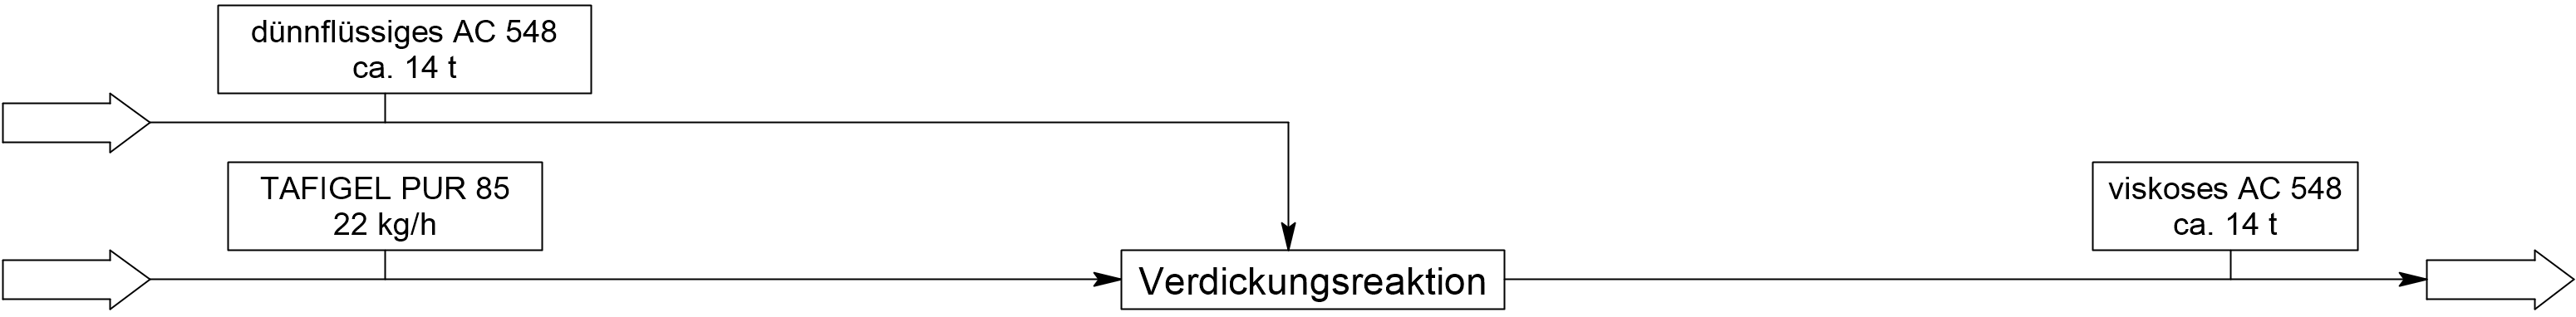
\includegraphics[width=0.75\textwidth]{img/verfahren_v1}
	\caption{Variante 1: ohne Vorbereitung}
	\label{fig:verfahren_v1}
\end{figure}
\FloatBarrier
%Ende
\begin{figure}[h!]
	\centering
	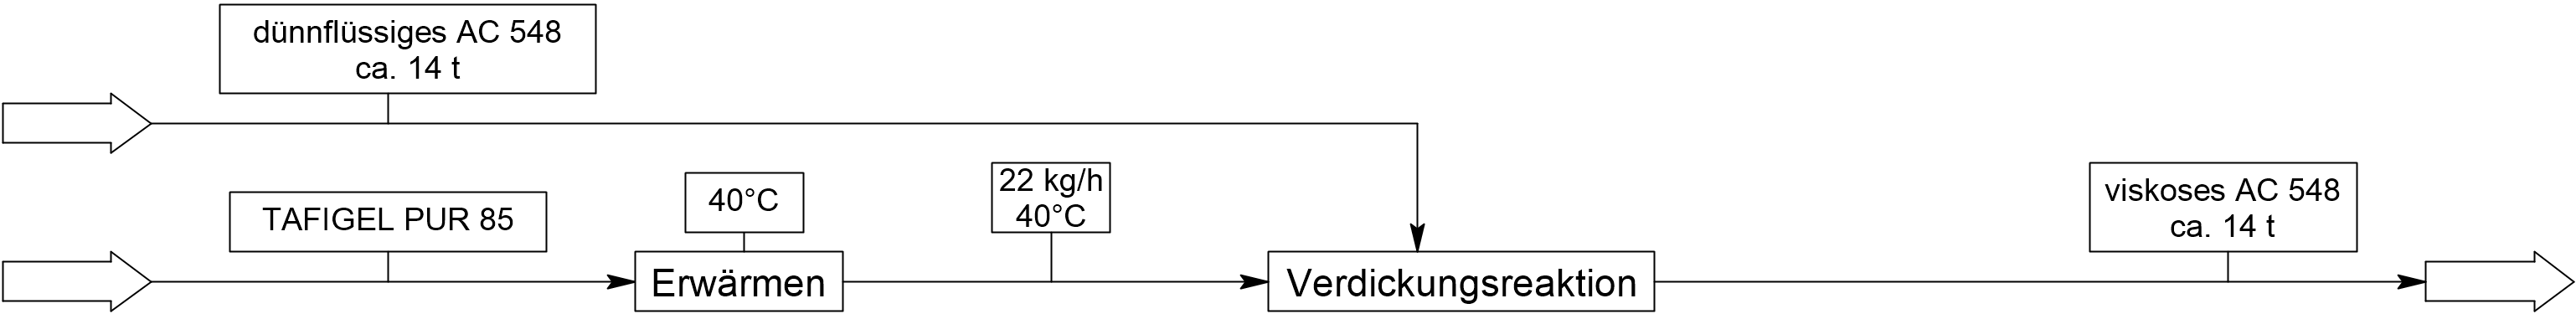
\includegraphics[width=0.75\textwidth]{img/verfahren_v2}
	\caption{Variante 2: mit Erwärmung des Verdickungsmittels und warmer Förderung}
	\label{fig:verfahren_v2}
\end{figure}
\FloatBarrier
%Ende
\begin{figure}[h!]
	\centering
	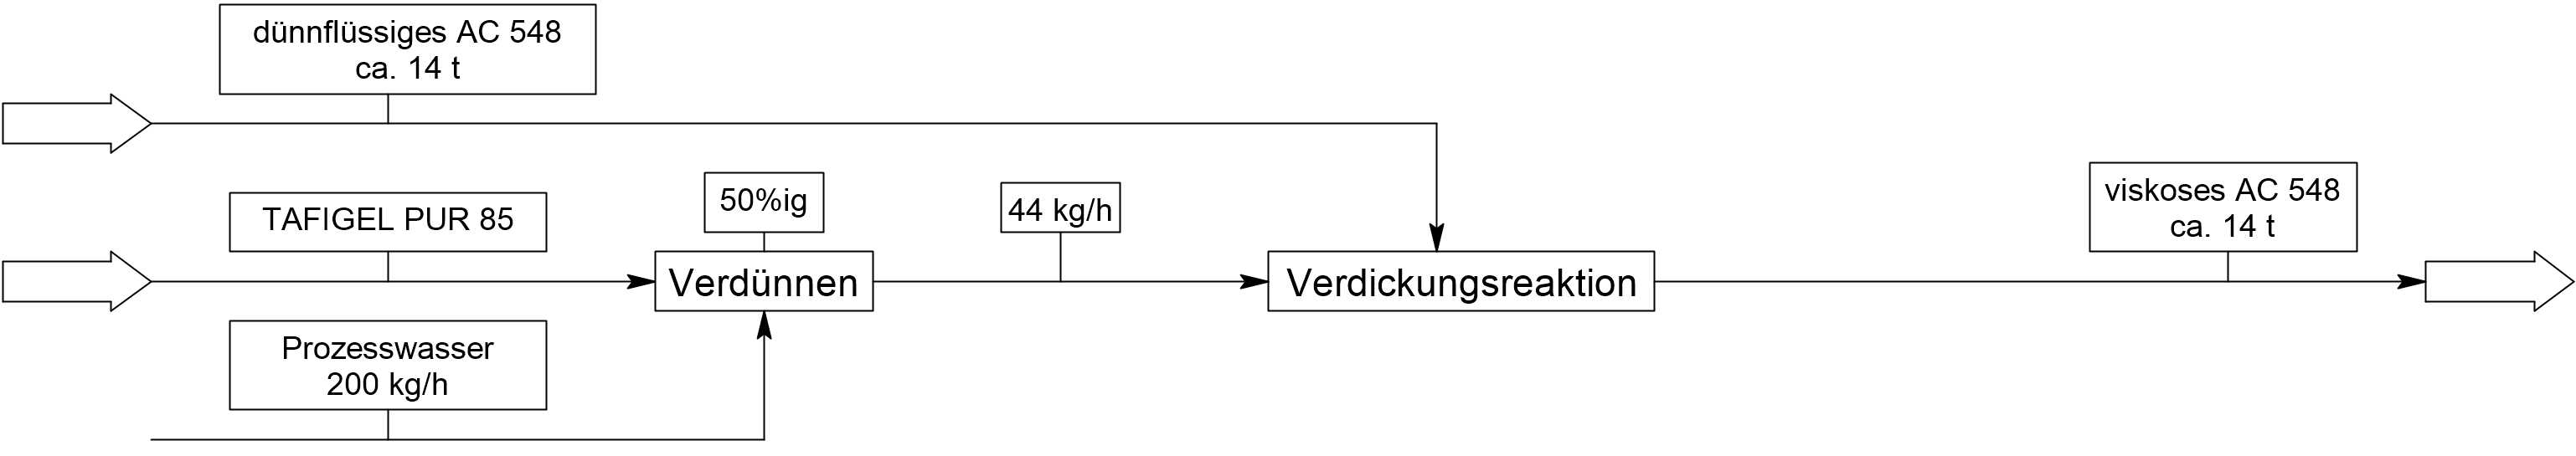
\includegraphics[width=0.75\textwidth]{img/verfahren_v3}
	\caption{Variante 3: mit Verdünnen des Verdickungsmittels}
	\label{fig:verfahren_v3}
\end{figure}
\FloatBarrier
%Ende
\begin{figure}[h!]
	\centering
	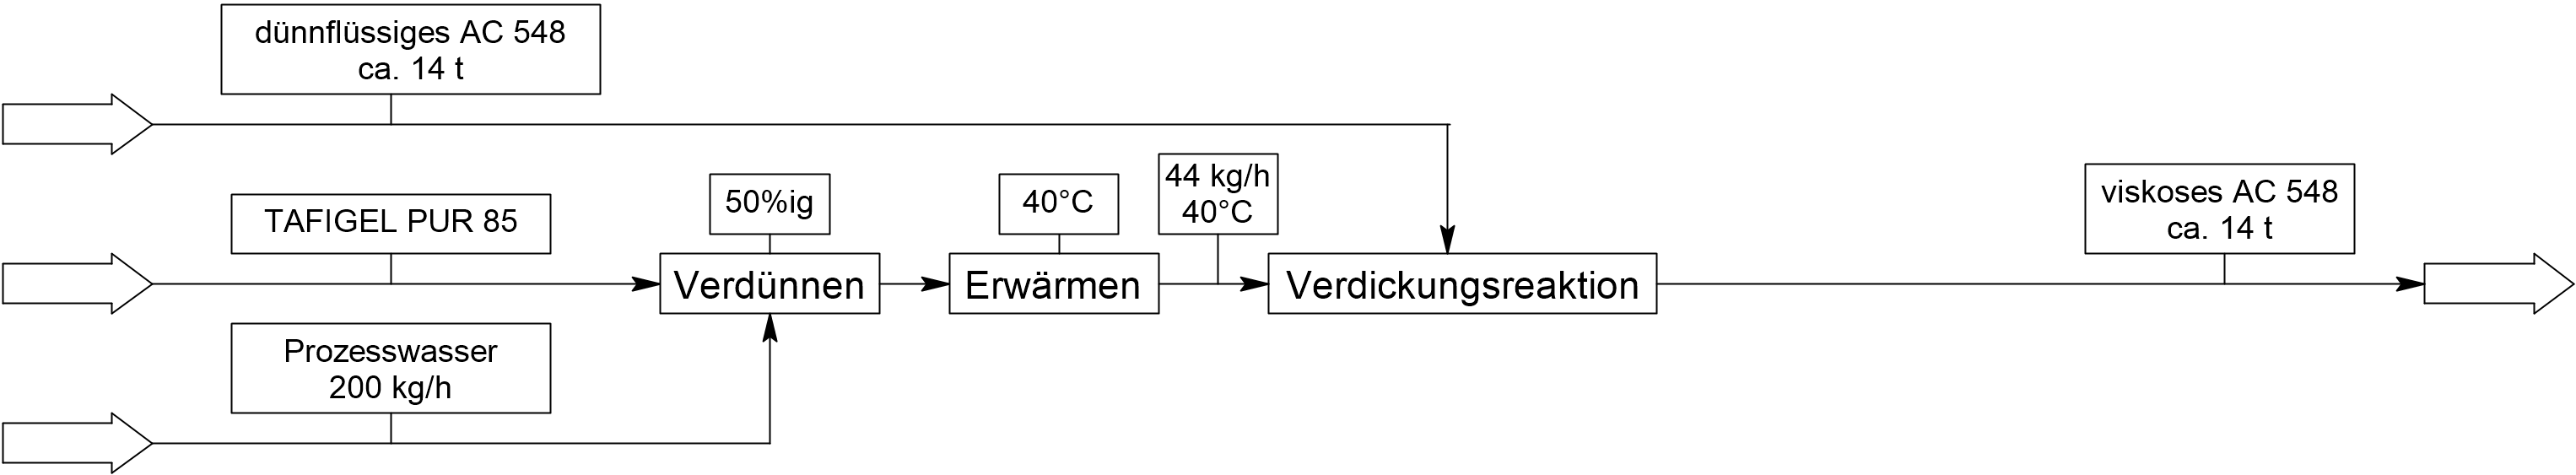
\includegraphics[width=0.75\textwidth]{img/verfahren_v4}
	\caption{Variante 4: mit Verdünnen und Erwärmen des Verdickungsmittels, sowie warmer Förderung}
	\label{fig:verfahren_v4}
\end{figure}
\FloatBarrier
%Ende\\

In Tabelle \ref{esm:grundverfahren} sind nun in Form einer Entscheidungsmatrix die vier verschiedenen Verfahrensvarianten verschiedenen Kriterien gegenübergestellt. Hierbei erfolgte subjektiv eine Einschätzung der Konsequenzen des Verfahrens anhand des jeweils betrachteten Kriteriums. Bis auf die \textit{Anzahl der Prozessschritte} gilt hierbei je höher der angegebene Konsequenzwert ist, desto höher fällt die Gewichtung für eine Positive Entscheidung der jeweiligen Variante. Die Summe der gewichteten Nutzenwerte einer Variante ist dann in der letzten Spalte der Matrix zu erkennen. 



% Table generated by Excel2LaTeX from sheet 'Daten'
\begin{table}
	\begin{adjustbox}{max width=\textwidth}
	\begin{threeparttable}
	\renewcommand*{\arraystretch}{1.2}
	\centering
	%\rowcolors{2}{white}{gray!25}
	\caption{Entscheidungsmatrix - Grundverfahren}
	\label{esm:grundverfahren}
		\begin{tabular}{l|l|c|c|c|cccc|cccc|cccc}
			\hline
			\multicolumn{5}{c|}{}&\multicolumn{4}{c|}{\textbf{Bewertung}}	&  \multicolumn{4}{c|}{\textbf{Erfüllungsstatus} $\left[\si{\percent}\right]$} & \multicolumn{4}{c}{\textbf{gewichteter Erfüllungsstatus} $\left[\si{\percent}\right]$}\\
			\hline
			\textbf{Kategorie} & \textbf{Kriterium} & \textbf{Gewichtung $\left[\si{\percent}\right]$}& \textbf{Bmin}&\textbf{Bmax}&\textbf{V1} & \textbf{V2} & \textbf{V3} & \textbf{V4} & \textbf{V1} & \textbf{V2} & \textbf{V3} & \textbf{V4}& \textbf{V1} & \textbf{V2} & \textbf{V3} & \textbf{V4}\\
			\hline
			Prozessdesign & Anzahl der Prozessschritte 		&15,0 	&0&1	&1&0,5&0,5&$0,\overline{3}$&100&50&50&33	&15,0&7,5&7,5&5,0\\
			Prozessdesign&Dosiergenauigkeit					&15,0	&0&2	&0&1&2&2&0&50&100&100	&0,0&7,5&15,0&15,0\\
			Hygiene & Sauberkeit Anlagenkomponenten 		&20,0	&0&2	&2&1&0&0&100&50&0&0		&20,0&10,0&0,0&0,0\\
			Hygiene&Spülbarkeit der Leitungen				&20,0	&0&2	&0&1&2&2&0&50&100&100	&0,0&10,0&20,0&20,0\\
			Investition& Isolierung/Beheizung der Leitung	&7,5	&0&1	&1&0&1&0&100&0&100&100	&7,5&0,0&7,5&7,5\\
			Investition&Höhe des Förderdrucks				&7,5	&0&2	&0&1&2&2&0&50&100&100	&0,0&3,8&7,5&7,5\\
			Investition&Notwendigkeit eines Rührers			&7,5	&0&3	&3&2&1&0&100&67&33&25	&7,5&5,0&2,5&0,0\\
			Investition&Notwendigkeit eines Vorlagebehälters&7,5	&0&3	&3&2&1&0&100&67&33&25	&7,5&5,0&2,5&0,0\\
			\hline	
			\multicolumn{2}{r|}{\textbf{Summe}}	& 100,0 & \multicolumn{10}{c|}{ } & 57,5 &48,8&62,5&55,0\\
			\hline
	\end{tabular}
	\begin{tablenotes}[flushleft]
		\footnotesize
		\NumTabs{6}
		\item Anzahl der Prozessschritte: \tab\tab reziproke Anzahl der Schritte  \tab (1 = ein Schritt; 0,5 = 2 Schritte; ...)
		\item Dosiergenauigkeit: \tab\tab 2 - höher, \tab 1 - mittel, \tab 0 - niedriger
		\item Sauberkeit Anlagenkomponenten: \tab 2 - hygienisch, \tab 1 - teilweise hygienisch, \tab 0 - unhygienisch
		\item Spülbarkeit der Leitungen: \tab\tab 2 - gut spülbar, \tab 1 - spülbar, \tab 0 - schlecht spülbar
		\item Isolierung/Beheizung der Leitungen: \tab 1 - nicht nötig, \tab 0 - nötig
		\item Höhe des Förderdrucks: \tab\tab 2 - niedriger, \tab 1 - mittel, \tab 0 - höher
		\item Notwendigkeit eines Rührers: \tab\tab 3 - nicht nötig, \tab 2 - bedingt nicht nötig, \tab1 - bedingt nötig, \tab 0 - nötig
		\item Notwendigkeit eines Vorlagebehälters: \tab 3 - nicht nötig, \tab 2 - bedingt nicht nötig, \tab1 - bedingt nötig,\tab 0 - nötig
	\end{tablenotes}
\end{threeparttable}
\end{adjustbox}
\end{table}%
\FloatBarrier



Es zeigt sich, dass Variante 1 mit \SI{39}{\percent} höchster Anteil, die Varianten 2 und 3 mit nahe zu gleichen Werten von 22 und \SI{23}{\percent} sind im mittleren Bereich und die Variante 4 mit dem geringsten Anteil von \SI{17}{\percent}. Die primäre Entscheidung liegt demnach laut Tabelle \ref{esm:grundverfahren} bei Variante 1 der direkten Dosierung ohne weitere Vorbereitungen.


%Skala:
%Eignung
%5 ja 
%4 bedingt ja 
%3 bedingt
%2 bedingt nein
%1 nein

%Kriterien:
%Sauberkeit
%Anzahl der Prozessschritte
%Kosten
%Viskositätsveränderung
%Vorlagebehälter nötig ?

Aus 

\subsubsection{Entscheidung für Gebindetyp}
%Preis nachfrage
%\subsubsection{Angebotsanfrage}
%\subsubsection{Entscheidungsverfahren}

\subsubsection{Entscheidung für Pumpendosierung oder Dosierbehälter}

\subsubsection{Auswahl des Pumpentyps}
%\subsubsection{Literaturarbeit}
%Bücher gelesen für Auswahlhilfe
%\subsubsection{Fachgespräche und Angebotsanfrage}
%\subsubsection{Entscheidungsverfahren}

%\subsection{Auswahl des Pumpentyps, sowie des Leitungsdurchmessers}
%Gespräche geführt und Leitung hat sich nach möglichen Drücken in der Anlage und Pumpentyp, sowie Berechnungen gerichtet gerichtet

\subsubsection{Auswahl des Messverfahrens}

\subsection{Technische Planung für Verdickungsmitteldosierung}
\subsubsection{Verfahrensfließbild der Verdickerdosierung}
\subsubsection{R\&I- Fließbild der Verdickerdosierung}
\subsubsection{Rohrleitungsplanung der Verdickerdosierung}
%vertretbarer Druckverlust
%Rohrdurchmesser und Nenndruck
%--> Rohrleitungsklassifizierung

\subsubsection{EMSR-Plan der Messtechnik für die Dosierung}

\subsection{Gefährdungsbeurteilung der geplanten Verdickungsmitteldosierung}


